%\section[]{Introduction}

\begin{comment}
\begin{frame}
\frametitle{Contexte scientifique}

\begin{columns}
\begin{column}{0.7\textwidth}
\begin{maliste}
\item Cadre th\'eorique : Mod\`ele Standard\\
$\rightarrow$ consolid\'e avec d\'ecouverte boson scalaire
\vspace*{0.2cm}
\item LHC : test \`a des \'energies nouvelles
\vspace*{0.2cm}
\item Modèle Standard incomplet
\begin{itemize}
\item Gravitation, matière noire
\item Origine mécanisme EWSB
\item ...
\end{itemize}
\vspace*{0.2cm}
\item Naturalit\'e $\rightarrow$ $\Lambda_\text{SM}\simeq$TeV
%This  is  not  in  itself  a  proof  that  new  particles  must  be  present  in  the  energy regime of the LHC and other planned accelerators.  But, it indicates a tremendous opportunity for discovery.
\end{maliste}
\end{column}
\begin{column}{0.5\textwidth}
\begin{center}
\includegraphics[width=0.8\textwidth]{Figures/FourTops/Fig_particles_and_interactions.png}
\end{center}
\end{column}
\end{columns}

\begin{center}
\includegraphics[width=0.5\textwidth]{Figures/FourTops/ParticleAcceleratorVsYears.png}
\end{center}

\end{frame}
\end{comment}

\begin{frame}
\frametitle{Run 1 du LHC}

\vspace*{-0.1cm}
\begin{center}
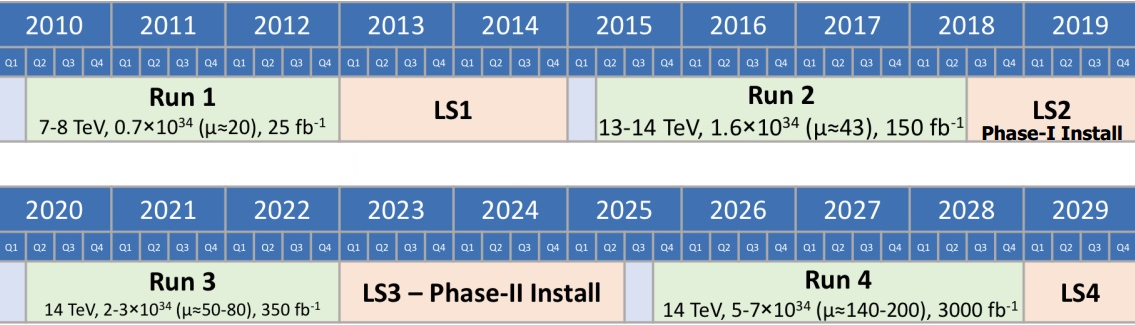
\includegraphics[width=0.8\textwidth]{Figures/Intro/LHCrunplan_modif.png}
\end{center}

\begin{small}
\begin{maliste}
\item Activités sur \ATLAS{} entre 2008 et 2015
\vspace*{0.1cm}
\begin{itemize}
\item 2008 - 2009 puis 2011 $\rightarrow$ 2015 : recherche de nouvelle physique
\vspace*{0.05cm}
\item 2009 $\rightarrow$ 2012 : calibration des jets
\vspace*{0.05cm}
\item Interpr\'etation statistique
\end{itemize}
\vspace*{0.1cm}
\item Co-encadrement de 2 doctorants
\end{maliste}
\end{small}

\begin{center}
\includegraphics[width=0.38\textwidth]{Figures/Intro/sumLumiByWeek.png}
\includegraphics[width=0.38\textwidth]{Figures/Intro/intlumivstime2012DQ.png}
\end{center}
\end{frame}

\begin{frame}
\frametitle{D\'etecteur ATLAS}

\begin{center}
\vspace*{-0.3cm}
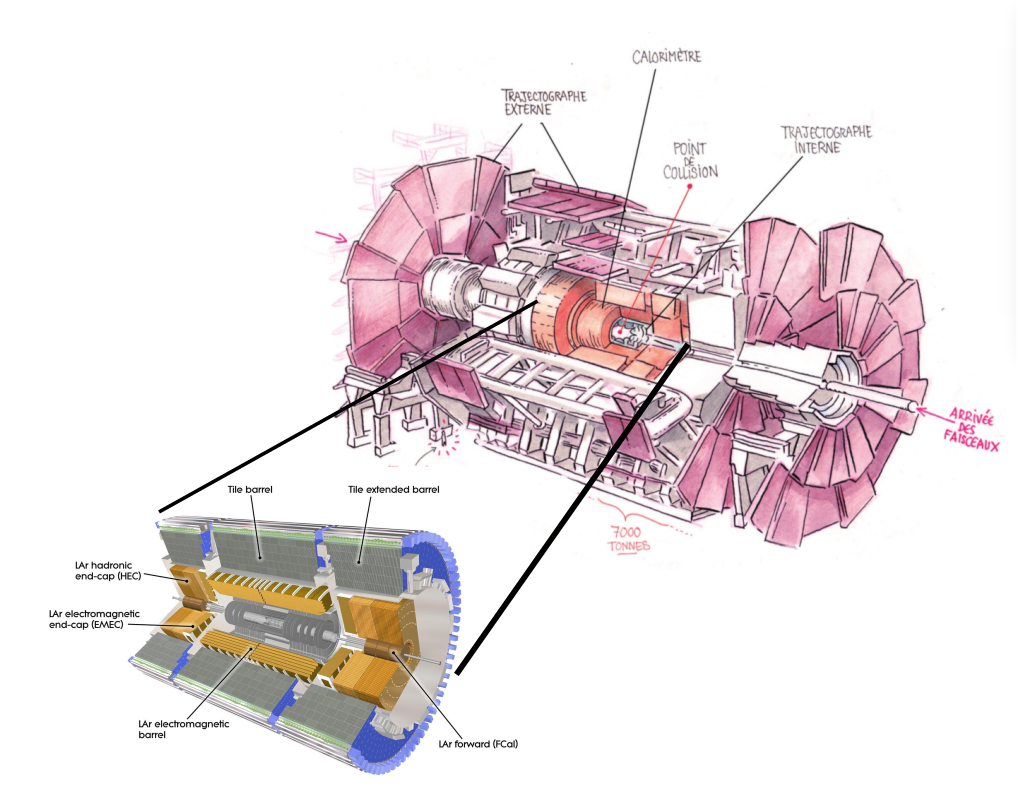
\includegraphics[width=1\textwidth]{Figures/Intro/ATLAS_full.png}
\end{center}

\end{frame}

